% Macro Definitions for Operators used in this file
\newcommand{\loft}[5]{\ensuremath{\Omega{\bf \mathcal{L}}_{#1}^{#2,#3} [\{#4\} (#5)]}}
\newcommand{\affine}[5]{\ensuremath{\Delta{\bf \mathcal{A}}_{#1}^{#2,#3} [\{#4\} (#5)]}}
\newcommand{\boolop}[5]{\ensuremath{\Omega{\bf  \mathcal{B}}_{#1}^{#2,#3} [\{#4\} (#5)]}}
\newcommand{\generic}[7]{\ensuremath{#1{\bf \mathcal{#2}}_{#3}^{#4,#5} [\{#6\} (#7)]}}


\section{New Form Features Representation}

{\em Form Features} come in different flavors in different CAD applications. Even within same application, similar looking features are presented in different ways e.g.  {\em Fillet} and {\em Chamfer}, both are similar in the sense that they both operate on an edge-chain, take size parameter and generate curved or planar face respectively. Topologically both are exactly same. So if one takes curved-or-planar as an argument, both operations can be modeled as a single operator. Following section proposes a set of core operators that would cater to most of the {\em Form Features} available in CAD applications. 

Snyder \cite{Snyder1992} mentioned that a limited set of shapes can be generated using {\em Sweep}. A {\em Sweep} is an operator where moving a shape (called {\em generator}) along a trajectory (called {\em guide curve}) creates variety of shapes. It presents a natural, intuitive way for creation of shapes. {\em Sweep}, by its strict meaning, is limited by use of a single profile. A more generic operation would be {\em Loft}, where multiple profiles are joined together, along a guide curve. It is found that most of the primitives like {\em Box, Cylinder, Cone, Torus, Sphere} and operators like {\em Extrude, Revolve, Sweep, Loft}, in their simplistic form, can be modeled using a {\em Loft} operator. Though externally these features manifest themselves in different forms, underlying kernel operation could be just one, i.e. a generic {\em Loft}.

Similarly, operators like {\em Translation, Rotation, Scaling} can be modeled using one generic {\em Affine Transformation} operator. {\em Pattern, Mirror} can also be modeled using the same by taking an additional argument as {\em number of copies}.

Another set of operators that can be uniquely represented as a single operator are {\em  Boolean} operators. {\em Union, Difference, Intersection} work on one {\em target body} and multiple {\em tool bodies} with a difference of only  'which cells to retain' logic.

Such set of core operators has lots of advantages like:
\begin{enumerate}
\item Operators can be agnostics to the CAD applications. CAD applications may call them differently but the kernel calls could be same.
\item Data interoperability could be easier as operators are few, neutral and standardized.
\item Algorithms based on them can be easily ported to different applications, e.g. Midsurface Extraction developed on such core operators can then be ported to in any CAD-CAE application honoring them.
\end{enumerate}

In many CAD applications, operators are presented as a combination, e.g. {\em  Extrude}, apart from parameters such as {\em sketch} and {\em direction-length}, can ask choice of {\em boolean} and {\em draft-angle}. In the representation scheme presented below, internal {\em booleans} are decoupled from the {\em feature} and are modeled separately  i.e. {\em Extrude} will create just the {\em tool body} which will be {\em boolean-ed} later.

Representation scheme used in this paper is largely based upon Interactive Configuration Exploration  (ICE) scheme developed by Moustapha \cite{Hoda2005}. Although some fundamental entities, syntaxes are borrowed from ICE, we attempt to enhance the set of entities as well as operators for formulating {\em form features} and the derived application {\em feature}, {\em Midsurface}.

\subsection{ICE scheme}
{\em "The ICE notation is a formalism for describing shapes and  configurations,  by  means  of  their  generative  and  relational  structures"} \cite{Hoda2005}.  There are two fundamental entities in ICE, one is a {\em point} shown as $\bar{p}$ and another is called {\em Regulator}, which is an abstraction that represents a unit of action like transformation, constraints, relations etc . A generic {\em Regular} is represented as 

{\Large \generic{category}{R}{instance}{subtype}{dimension}{arguments}{shapes}}

	 For example ,

	\affine{}{T}{1}{\bar{p},\bar{t},d,n}{shape} 

	where,

		 $\Delta$ : Transformation category\\
	     	 ${\bf \mathcal{A}}$ : Affine Transformation regulator\\
		 $^T$: subtype Translation \\
		 $^1$ : along line (1 dimensional)\\
	         $\bar{p}$ : reference point\\
  		 $\bar{t}$ : vector\\
		 $d$ : distance\\
		 $n$ : number of copies\\
		 $shape$ : the shape which is moving

Notation norms:
\begin{enumerate}

	\item {\em Regulators} are in {\bf bold}, {\bf  $\mathcal{R}$} , represents a unit of action
	\item {\em shapes} are in {\em lowercase}, say, {\em circle, profile}
	\item Prefix to a  {\em Regulator} is its {\em category}, like, \\
		 $\Delta$	 :  transformations  \\
		 $\Phi$		 :  constraints  \\
		 $\Psi$		 :  hierarchies  \\
		 $\Pi$		 :  topologies  \\
		 $\Xi$		 : variations  \\
		 $\Omega$	:  operations

	\item Superscripted$^{suffixes}$  indicate  regulator  {\em subtype},  for instance, $\Delta C^p$ and  $\Delta C^e$  respectively specify parabolic and elliptical curve regulators

	\item Numerical$^{suffixes}$ denote the dimension of the {\em Regulator}, for instance, $\Delta M^0$ ,   $\Delta M^1$ , and   $\Delta M^2$, respectively represent a mirror point (0-dimensions), a mirror line (1-dimension) and a mirror plane (2-dimensions)

	\item  Subscripted$_{suffixes}$ for {\em Regulators,  shapes} represent  as  indices;  for  example  $\Delta T_1$ ,  and  $\Delta T_2$  are  two different instances of {\em Translation Regulators} used in the same configuration.

	\item {\em Regulators} can be generative or non-generative.  Generative  regulators (depicted by the presence of the “ n ” parameter)  take  an  input  shape  and  create output  shapes,  while  non-generative  regulators  act  on  the  input  shape.

	\item $\Delta {\bf T}(\bar{s})^{<0><1><2>}$  is  a  discrete  application  generating disjoint points, while  $\Delta  {\bf T}(\bar{s})^{<0,1,2>}$  is a continuous application generating a line.  

	\item Key-points ($ e$ : endpoint,   $m$ : midpoint,   $s$ : start-point) To access key-points (such as the midpoint): $ shape_A \langle m_1 \rangle$, length by $shape_A \langle l \rangle$

	\item These notations are extended as follows to incorporate few more necessary syntactical elements\\
		$child::parent$ : subclass relationship\\
		$|$ : logical OR\\
		$\&$ : logical AND\\
\end{enumerate}

\subsection{Form Features extensions to ICE}

Some of the fundamental entities like {\em point}, {\em line} are already defined in ICE but entities pertinent to Mechanical CAD, like {\em profile}, {\em sketch} have been added newly in this paper. Also, extending ICE, this paper proposes use of class hierarchy, i.e. {\em child::parent} relationships between entities. Operators can leverage this arrangement by defining themselves in terms of the {\em parent} entities so that the operations are  applicable to any of the {\em child} classes as well.


\subsubsection{Entities ($\mathcal{E}$)}
In ICE, fundamental primitive is a {\em point}. All other geometric  entities are directly or indirectly defined in terms of points. Representation of each entity includes the dimension, 1 for {\em curves}, 2 for {\em surfaces} and 3 for {\em volumes}. 

\begin{enumerate}

\item {\bf Shape} ($shape$): A base class. All other entities directly or indirectly derive from it.

\item {\bf Point} ($point::shape$): A fundamental primitive expressed as $\bar{p}$. 	

\item {\bf Line} ($line::curve$): Defined by two points ($\bar{p}$ and $\bar{s}$), distance $d$ apart and is expressed in terms of {\em Translation} as \affine{}{T}{1} {\bar{p},\bar{t}, d,n} {\bar{s} )^{<1>} }	

\item  {\bf Arc} ($arc::curve$): Defined by three points, embedding angle $\theta$ and is expressed in terms of {\em Rotation} as \affine{}{R}{1} {\bar{p},\bar{t}, \theta,n} {\bar{s} )^{<0-1>}}	

\item {\bf Circle} ($circle::curve$) An $arc$ with full rotation, thus having $\theta = 360$ and is expressed as \affine{}{R}{1} {\bar{p},\bar{t}, 360,n} {\bar{s} )^{<0-1>}} 

\item {\bf Curve} ($curve::shape$): A generic entity modeled in terms of $n$ points expressed as \affine{}{C}{1} {\bar{p},\bar{t}, d,n} {\bar{s} )^{<0-1>}} 

\item {\bf Polygon} ($polygon::shape$): Collection of $n$ connected $line$ segments and is expressed as \generic{\Pi}{C}{}{P}{1}{C_0}{line)^{<0-n>}}	

\item {\bf Profile} ($profile::shape$): Collection of $n$ connected $curve$ segments and  is expressed as \generic{\Pi}{C}{}{P}{1}{C_0}{curve)^{<0-n>}} 

\item {\bf Sketch} ($sketch::shape$): Collection of $profiles$, first outer and rest  inner  and is expressed as \generic{\Pi}{C}{}{P}{1}{C_0}{profile)^{<0><1-n>}}		

\item {\bf Ruled Surface} ($ruledSurface::shape$): Sweeping of a line along a curve and is expressed as \affine{}{T}{2} {\bar{p},\bar{t}, d,n} {curve{^{<0-1>} }}	

\item {\bf Surface} ($surface::shape$): Modeled using collection of $U,V$ curves	and is expressed as \affine{}{C}{2} {\bar{p},\bar{t}, d,n} {curve{^{<0-1>} }}   

\item {\bf Solid} ($solid::shape$): Modeled using two generic surfaces way in third $w$ direction and is expressed as \affine{}{C}{3} {\bar{p},\bar{t}, d,n} {surface{^{<0-1>} }} 	

\end{enumerate}

%-----------------------------------------------------------------------------------------------------------------------------------------------------

\subsubsection{Affine Transformation Operators ($\mathcal{A}$)}

{\em Affine Transformations} use matrix multiplications and can be performed on entities of various dimensions, like $point (0)$, $curves(1)$, $surface(2)$ and $solid(3)$. All these are generically clubbed together under {\bf $\mathcal{A}$} with subtypes as $T,R,S$ for {\em Translation}, {\em Rotation} and {\em Scaling} respectively.


\begin{enumerate}
\item {\bf Translation} moves $shape$, by distance $d$, in direction $\bar{t}$, from point $\bar{p}$ and is expressed as 	\affine{}{T}{0|1|2|3 }{\bar{p},\bar{t}, d,0} {shape}
\item{\bf Rotation} rotates $shape$, by angle $\theta$, about point $\bar{p}$ and is expressed as 	\affine{}{R}{0|1|2|3 }{\bar{p},\bar{t}, \theta,0} {shape}	
\item {\bf Scaling} scales $shape$, by factor  $f$, about an axis $\bar{p},\bar{t}$ and is expressed as 	\affine{}{S}{0|1|2|3 }{\bar{p},\bar{t}, f,0} {shape}		
\end{enumerate}

%-------------------------------------------------------------------------------------------------------------------------------------------------------------------------------------
Copy commands like {\em Pattern}, {\em Mirror} can be modeled as {\em Affine Transformations} with $n$ copies.

\begin{enumerate}
\item {\bf Linear Pattern} copies $shape$ linearly and is expressed as \affine{}{T}{0|1|2|3 }{\bar{p},\bar{t}, d,n} {shape} 
\item {\bf Circular Pattern} copies $shape$ circularly and is expressed as \affine{}{R}{0|1|2|3 }{\bar{p},\bar{t}, \theta,n} {shape} 
\item {\bf Mirror} makes a single copy, mirror-ed about $\bar{t}$ and is expressed as \affine{}{M}{0|1|2|3 }{\bar{p},\bar{t}, 0,1} {shape}	
\end{enumerate}

\subsubsection{Boolean Operators ($\mathcal{B}$)}

%-------------------------------------------------------------------------------------------------------------------------------------------------------------------------------------
Boolean operations are also generic in the sense that they can apply on any $shape$ of dimensionalities like $curves(1)$, $surface(2)$ and $solid(3)$. 
Here first shape $shape_0$ is regarded as {\em target body} and result of the operation is stored in it. Rest of the shapes are termed as {\em tool bodies}.

\begin{enumerate}
\item {\bf Union} combines all the tool shapes ${shape_{1-k}}$ into master shape $shape_0$ and is expressed as	\boolop{}{U}{1|2|3 }{} {shape_{0-k}} 	
\item {\bf Difference} removes combination of all the tool shapes ${shape_{1-k}}$ from master shape $shape_0$ and is expressed as	\boolop{}{D}{1|2|3 }{} {shape_{0-k}}  
\item {\bf Intersection} keeps only common portion of the shapes ${shape_{0-k}}$ into master shape $shape_0$ and is expressed as	\boolop{}{I}{1|2|3 }{} {shape_{0-k}} 	 
\end{enumerate}


%---------------------------------------------------------------------------------------------------------------------------------------------------------------------------------------------
\subsubsection{Loft Operators ($\mathcal{L}$)}

Loft is a generic operator (Figure \ref{figure_Loft})  capable of generating most of the basic shapes. It joins {\em profiles} along a guide {\em curve}. 

\begin{figure}[htbp]
%\begin{tabular}{  p{0.22\textwidth}  p{0.22\textwidth} }

	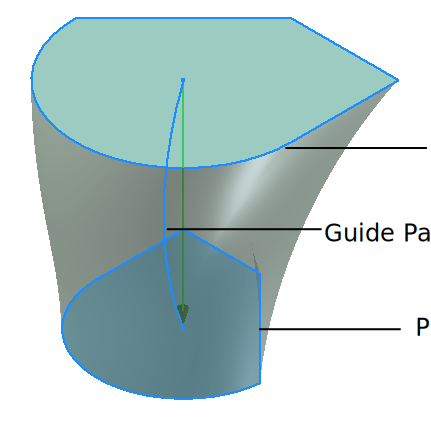
\includegraphics[scale=0.35]{../Common/images//LoftPreview.pdf} 
	%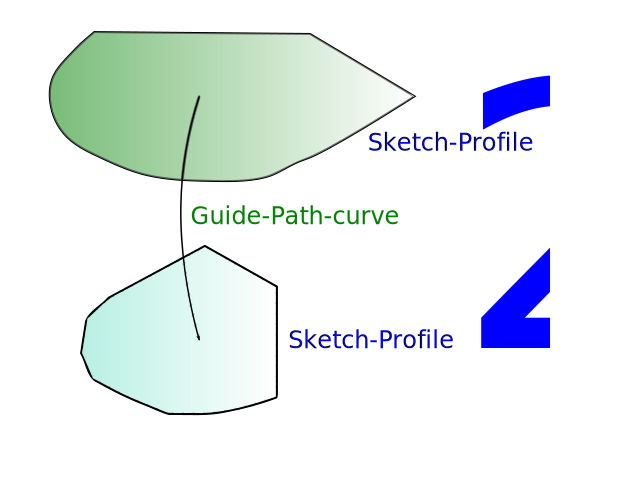
\includegraphics[scale=0.3]{../Common/images//LoftProfilesPath.pdf} \\

%\end{tabular}
\caption{Generic Loft feature}
\label{figure_Loft}
\end{figure}

Represented as:
\loft{}{subtype}{3}{curve, 0 | C_{0,1,2}}{ (sketch )^{<1-n>}}

{\em Continuity} options like $C_0$ for connectedness, $C_1$ for tangency and $C_2$ for curvature continuity can be specified at the ends where this body joins the existing shape. 
In case this body is disjoint or is the first one in the scene, no {\em continuity}  is specified. 

Some {\em form features} also specify a {\em draft-angle}  for tapering sides. This can be modeled as {\em Loft} between two {\em profiles}, where the second {\em profile} is offset-ed inside-or-outside. 

Output of the Loft can either be $solid$ (where capping faces are put to close the shape) or $surface$ (capping faces are not put) and accordingly dimensionality of $2|3$ can be specified.


\begin{figure}[htbp]
	\includegraphics[scale=0.35]{../Common/images//LoftExtrudeRevSwp.pdf} 
\caption{Extrude, Revolve and Sweep in terms of Loft}
\label{figure_extrevswp}
\end{figure}

{\bf Loft} can manifest itself in different forms (Figure \ref{figure_extrevswp}) as elaborated below:
%----------------------------------------------------------------------------------
\begin{enumerate}
\item {\bf Extrude without draft} is denoted by $EnD$ subtype, has single $sketch$, swept along a $line$ and is expressed as	\loft{}{EnD}{3 }{line, 0 | C_0}{ (sketch )^{<1>}}		
\item {\bf Extrude with draft} is denoted by $EwD$ subtype, has two $sketches$ between which loft is made along a $line$ and is expressed as \loft{}{EwD}{3 }{line, 0 | C_0}{ (sketch )^{<1-2>}}	
\item {\bf Revolve without draft} is denoted by $RnD$ subtype, has single $sketch$, swept along a $arc$ and is expressed as	\loft{}{RnD}{3 }{arc, 0 | C_0}{ (sketch )^{<1>}}		
\item {\bf Revolve with draft} is denoted by$ RwD$ subtype, has two $sketches$ between which loft is made along a $arc$ and is expressed as\loft{}{RwD}{3 }{arc, 0 | C_0}{ (sketch )^{<1-2>}}	
\item {\bf Sweep without draft} is denoted by $SnD$ subtype, has single $sketch$, swept along a $curve$ and is expressed as	\loft{}{SnD}{3 }{curve, 0 | C_0}{ (sketch )^{<1>}}		
\item {\bf Sweep with draft} is denoted by $SwD$ subtype, has two $sketches$ between which loft is made along a $curve$ and is expressed as \loft{}{SwD}{3 }{curve, 0 | C_0}{ (sketch )^{<1-2>}}	
\item A generic {\bf Loft} is $n$ profiles between which a loft is made along a generic $curve$ and is expressed as \loft{}{L}{3 }{curve, 0 | C_{0,1,2}}{ (sketch )^{<1-n>}} 
\end{enumerate}


%---------------------------------------------------------------------------------------------------------------------------------------------------------------------------

{\bf Primitive} shape operators are further specializations of {\bf $\mathcal{L}$} operators like {\em Extrude} and {\em Revolve}. By changing shape of the {\em profile} and {\em curve} one can get different standard primitives  (Figure \ref{figure_ExtrudeBoxCylCone}) .

\begin{figure}[htbp]
	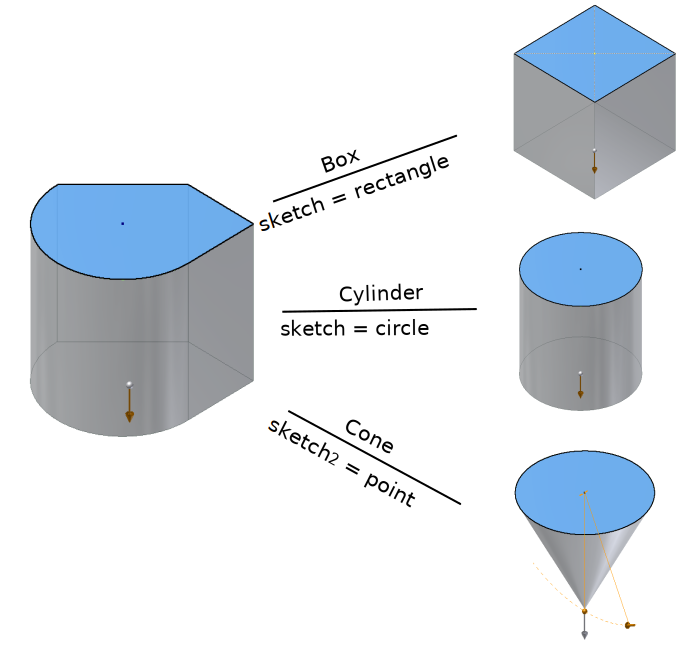
\includegraphics[scale=0.35]{../Common/images//ExtrudeBoxCylCone.pdf} 
\caption{Box, Cylinder, Cone in terms of Extrude-Loft}
\label{figure_ExtrudeBoxCylCone}
\end{figure}

\begin{enumerate}
\item {\bf Box} : {\em Extrude} with {\em Rectangle} as profile shape and is expressed as \loft{}{EnD}{3 }{line, 0 | C_0}{ (rectangle )}	
\item {\bf Cylinder} : {\em Extrude} with {\em Circle} as profile shape and is expressed as \loft{}{EnD}{3 }{line, 0 | C_0}{ (circle )}
\item {\bf Cone}: {\em Extrude with draft} with {\em Circle} as first profile shape, point as second and is expressed as \loft{}{EwD}{3 }{line, 0 | C_0}{ (circle, point)}
\item {\bf Torus} : {\em Revolve} with {\em Circle} as profile shape, arc as path and is expressed as \loft{}{RnD}{3 }{arc, 0 | C_0}{ (circle)}	
\item {\bf Sphere} : {\em Revolve} with {\em Circle} as profile shape, point as path and is expressed as \loft{}{RnD}{3 }{point, 0 | C_0}{ (circle)}	
\end{enumerate}

%---------------------------------------------------------------------------------------------------------------------------------------------------------------------------------
As demonstrated above, most of the {\em form features} used in CAD application can be modeled using  three operators, Affine Transformation ($\mathcal{A}$),  Boolean ($\mathcal{B}$) and Loft ($\mathcal{L}$), operating on Entities($\mathcal{E}$). This representation is called as {\bf $\mathcal{ABLE}$}. 

Other features like {\em Shell, Fillet, Chamfer} can be formulated using {\bf $\mathcal{ABLE}$}. With such a terse and expressive representation it is easier to define new, application specific features as well.  Following section demonstrates how{\bf $\mathcal{ABLE}$} can be used to express the Midsurface operator.



\subsection{Midsurface using $\mathcal{ABLE}$}

Most of the Midsurface Extraction algorithms work on geometry of the final shape, which can be in the form of {\em Mesh} or Boundary Representation ({\em Brep}) solid. Midsurfaces generated by these algorithms are still  not well connected and have problems like spurious surfaces, gaps etc. Very few (\cite{Hamdi2005}, \cite{Robinson2006} and \cite{Stolt2005}) have considered leveraging use of {\em feature} information in such algorithms, but their usage is limited to very basic {\em form features}. Some approaches (\cite{Boussuge2013a}) use decomposition of {\em Brep} solid to create {\em feature tree} like representation so that Midsurface can be worked out on simpler shapes.

In a {\em feature tree}, at each {\em feature} level, the operands (especially the {\em tool bodies}) are relatively simpler, thus making Midsurface Extraction more deterministic \cite{YogeshIITM2013}.  Use of Spatial Grammar has made it possible to come up with a terse representation (as demonstrated by $\mathcal{ABLE}$) so that algorithms need not have to work on all but just few generic operators. 

As  {\bf $\mathcal{A}$} operators do not change topology and geometry type, Midsurface generated can follow just the same transformation as that of the parent shape. We need to consider only  {\bf $\mathcal{L}$}  and  {\bf $\mathcal{B}$} operators for Midsurface (Figure \ref{figure_Midsurf}) generation. Advantage of the Spatial Grammar defined for Form Features is evident here. One does not need to decide rules for all features but just two - Loft and Boolean, and depending of different specifications they automatically become applicable to rest of the form features.

As for implementation, a {\em feature-based} CAD model is taken as an input. Using direct access or via Application Programming Interface (APIs), {\em feature tree} is queried. A {\em feature tree} is a chronological list of {\em features} stored as part gets built. Each {\em feature} is traversed one by one, and wherever applicable, a corresponding Midsurface is extracted. For {\em features} like {\em Extrude} which may have internal-{\em boolean}, two separate {\em features} are modeled, one for {\em tool body} creation by {\em Extrude} and the second one as {\em Boolean}.

For {\em features} based on {\bf $\mathcal{L}$} operator, {\em feature} parameters such as {\em sketches-profiles}, {\em curve} etc are extracted first and then, based on rules specified below, Midsurface is generated.

\begin{enumerate}

\item {\bf Midcurve} is a set of {\em curves} representing abstraction of 2D {\em profiles}.	Methods like MAT \cite{Ramanathan2004}, Chordal Axis Transform (CAT) \cite{Quadros2008}, Straight-Skeleton \cite{Haunert2004} can be used. It is expressed as 	\generic{\Omega}{M}{}{C}{1}{d} {sketch} 

\item {\bf Midsurface} rules differ based on relative sizes of {\em profiles} and {\em curve}.
\begin{enumerate}
\item {\bf Thin Profile}  (Figure \ref{figure_MidsurfSmallProfile}): If {\em profile} is very small compared to {\em curve} ( $sketch_{length} \ll curve_{length}$), then {\em midcurve} is extracted from the {\em sketch} (as mentioned above) and {\em Lofted} with same feature parameters as that of  {\bf $\mathcal{L}$}. This rule is expressed as \loft{}{L}{2}{curve, 0 | C_{0,1,2}}{midcurve^{1-n}} 

\begin{figure}[htbp]
\centering \includegraphics[scale=0.40]{../Common/images//MidsurfSmallProfile.pdf} 
\caption{sketch is far smaller than curve}
\label{figure_MidsurfSmallProfile}
\end{figure}

\item {\bf Thin Loft}  (Figure \ref{figure_MidsurfSmallCurve}):  If {\em profile} is very big compared to {\em curve} ($sketch_{length} \gg curve_{length}$), then {\em midcurve} is not extracted  but the {\em sketch} itself is {\em Lofted} along half of the {\em curve}. This rule is expressed as \loft{}{L}{2}{curve/2, 0 | C_{0,1,2}}{sketch}.

\begin{figure}[htbp]
\centering \includegraphics[scale=0.40]{../Common/images//MidsurfSmallCurve.pdf}
\caption{sketch is far bigger than curve}
\label{figure_MidsurfSmallCurve}
\end{figure}

\item {\bf Thick Profile}:   If {\em profile} is comparable in size to {\em curve}  ($sketch_{length} \approx curve_{length}$), then it is a thick shape and Midsurface is not generated.
\end{enumerate}
\end{enumerate}


For {\bf $\mathcal{B}$} operators rules (Table \ref{table_BoolMidsurf}) are devised depending on where the target and tools have Midsurface extracted already.

\begin{table}[htbp]
\begin{tabular}{  p{0.3\textwidth} p{0.1\textwidth} }

{\bf Union} : If both operands, {\em target} and {\em tool bodies} are thin, i.e. they already have Midsurfaces in them, we need to extend both and join at common intersection &	
\raisebox{-0.6in}{\includegraphics[scale=0.2]{../Common/images//Midsurf_unite.png} } \\
{\bf Difference-Thin} : If {\em target} is thin having Midsurface, then irrespective whether {\em tool bodies} are thick or thin, they cut the Midsurface of {\em target} & 
\raisebox{-0.6in}{\includegraphics[scale=0.2]{../Common/images//Midsurf_diffthin.png} } \\
{\bf Difference-Thick} : If both operands, {\em target} and {\em tool bodies} are thick, in case of through or blind hole like situation, {\em midcurves} of combined {\em profiles} is calculated and {\em Lofted} with {\em target} {\bf $\mathcal{L}$} operator parameters  & 
\raisebox{-0.6in}{\includegraphics[scale=0.18]{../Common/images//Midsurf_diffthick.png} } \\

\end{tabular}
\caption{Midsurface of Boolean Operators}
\label{table_BoolMidsurf}
\end{table}



